\documentclass{CSArticle}[english]
\usepackage{LCSsymbols}
\title{\textbf{Optimization TD5}}
\author{\textbf{Chensheng LUO,Yue WANG}\\Track 1, Group 1}
\date{March 22th 2022}
\def\xtd{\tilde{\xbs}}
\begin{document}
\MakeSimpleTitle


\section{Question 1}
\label{Q1}
\subsection{Code in MATLAB}
Following code is given by the professor,which exerce the initialisation of question.
\begin{lstlisting}[style=MATLAB]
clc ; clear
%% Problem settings
D=8; %dim_of_the_search_space
size_of_the_box=5 ;
m=-size_of_the_box*ones(1,D);      % Lower bound
M=+size_of_the_box*ones(1,D);      % Upper bound

prob = @f_sphere; %  cost function

%% Parameters for DE
N  = floor(10+sqrt(D));	% Population Size (heuristic)
% N = 10*D  ; Luxurious choice
G  = 150;	% No. of iterations
F  = 0.8;	% Scaling factor
C  = 0.7;	% crossover probability

%% Starting of DE
f = NaN(N,G);   % collection of Vector to store f(population_g)
P = NaN(N,D,G); % collection of Matrix to store P(population_g)
V = NaN(N,D,G); % collection of Matrix to store the mutant vector 
U = NaN(N,D,G); % collection of Matrix to store the trial solutions 

Pinit = repmat(m,N,1) + repmat((M-m),N,1).*rand(N,D);	% initial P

P(:,:,1)=Pinit;

for n = 1:N
    f(n,1) = prob(P(n,:,1));	% Evaluating f(population_1)
end
\end{lstlisting}

For the algorithm, we give the MATLAB code as followings, it's composed with 3 steps:\par
\begin{lstlisting}[style=MATLAB]
%% Iteration loop
tic;
for g=1:(G-1)
    % Step 1 Mutation
    for n=1:N
        to_select=1:D;
        to_select(to_select==n)=[];
   
        size_TS=size(to_select,2);
        r = to_select(randperm(numel(to_select),3));
        
        V(n,:,g+1)=P(r(1),:,g)+F*(P(r(2),:,g)-P(r(3),:,g));
    end
    
    % Step 2 Crossover
    for n=1:N
        I=randi([1,D]);
        for i=1:D
            if rand()<=C | i==I
                U(n,i,g+1)=V(n,i,g+1);
            else
                U(n,i,g+1)=P(n,i,g);
            end
        end
    end
  
    % Step 3 Selection
    for n=1:N
        U(n,:,g+1)=max(m,min(M,U(n,:,g+1)));
        if prob(U(n,:,g+1))<f(n,g)
            P(n,:,g+1)=U(n,:,g+1);
            f(n,g+1)=prob(U(n,:,g+1));
        else
            P(n,:,g+1)=P(n,:,g);
            f(n,g+1)=f(n,g);
        end
    end
end
calculation_time=toc;
\end{lstlisting}
And finally, we have performance evaluation. The optimal value is got as the minimum value of \verb|f|. 
\begin{lstlisting}[style=MATLAB]
%% Key results at the end of the optimisation
disp('=========== OPTIMAL SOLUTION')
fprintf("calculation time = %gs \n",[calculation_time])

[best_value,best_generation]=min(min(f));
[best_value,best_index]=min(f(:,best_generation));
best_solution=V(best_index,:,best_generation);
fprintf("The best solution is given at  %d th generation \n",[best_generation])
fprintf("At index n=%d \n",[best_index])
fprintf("With the value = %.6f \n",[best_value])
fprintf("At the position = [%s] \n",[num2str(best_solution)])

\end{lstlisting}

\subsection{Illustration with example}
By runing this code in with the function \verb|f_sphere|, we get the following solution:
\begin{lstlisting}[style=RESULT]
=========== OPTIMAL SOLUTION
calculation time = 0.0514277s 
The best solution is given at  145 th generation 
At index n=4 
With the value = 0.000215 
At the position = [1.0079      0.9946     0.99834      1.0006     0.99453     0.99946     0.99275     0.99354] 
\end{lstlisting}

First, the optimal value is given close to the end of all iterations, and the obtained solution is close to the true minimal $x=\Onebb$, with a value $f=0.000215 \approx 0$.(As we know in section \ref{Q2}, the optimal is $f=0$ at $x=\Onebb$). The algorithm is quite efficient with a calculation time of less than 0.1s. 

\section{Question 2}
\label{Q2}
\begin{equation}
    \verb|f_sphere|(x)={\left\| x-1_{1\times D} \right\| _2}^2, x_{min}=1_{1\times D}
\end{equation}
\begin{equation}
    \verb|f_nondiff|(x)=\left\| x-4_{1\times D} \right\| _2^{\frac{1}{2}}, x_{min}=1_{4\times D}
    \end{equation}
\begin{equation}
    \verb|f_nondiff2|(x)={\left\| x+4_{1\times D} \right\| _2}^{\frac{1}{2}}+{\left\| x-4_{1\times D} \right\| _2}^{\frac{1}{2}}-{\left\| 8_{1\times D} \right\| _2}^{\frac{1}{2}}, 
    x_{min}=4_{1\times D}, -4_{1\times D}
    \end{equation}
\begin{equation}
\begin{aligned}
    \verb|f_nondiff2asym|(x)&={\left\| x+4_{1\times D} \right\| _2}^{\frac{1}{2}}+{\left\| x-4_{1\times D} \right\| _2}^{\frac{1}{2}}-{\left\| 8_{1\times D} \right\| _2}^{\frac{1}{2}}-\epsilon \frac{1_{1\times D}\left( x^T-4_{D\times 1} \right)}{8D},\\
    x_{min}&=4_{1\times D}, -4_{1\times D}
    \end{aligned}
\end{equation}
\begin{equation}
    \verb|f_rastrigin|(x)=10D+\sum_{i=1}^D{\lambda ^2{x_i}^2-10\cos \left( 2\pi x_i \right)}\textbf{},
    x_{min}=0
\end{equation}


The interest is 

\begin{itemize}
    \item First function: study the performance of the algorithm when there exists an unique optimum where the function is differentiable
    \item Second function: study the performance of the algorithm when there exists an unique optimum where function is not differentiable 
    \item Third and the fourth function: study the performance of the algorithm when there are several optima where the function is not differentiable
    \item Fifth function: study the performance of the algorithm when the global optimum is unique, but there exist several local optima where the function is not differentiable at any optimum.
\end{itemize}


\begin{figure}[h!]
\centering
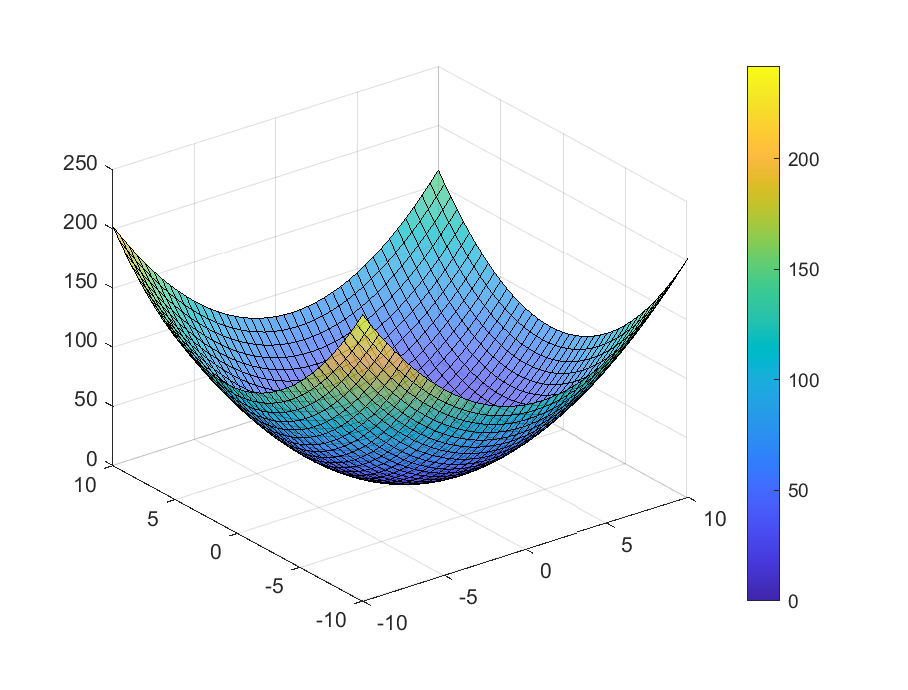
\includegraphics[scale=0.4]{figure/Q2-sphere.eps}
\caption{Image of function \text{f\_sphere}}
\label{fig:Q1_crite}
\end{figure}\par


\begin{figure}[h!]
\centering
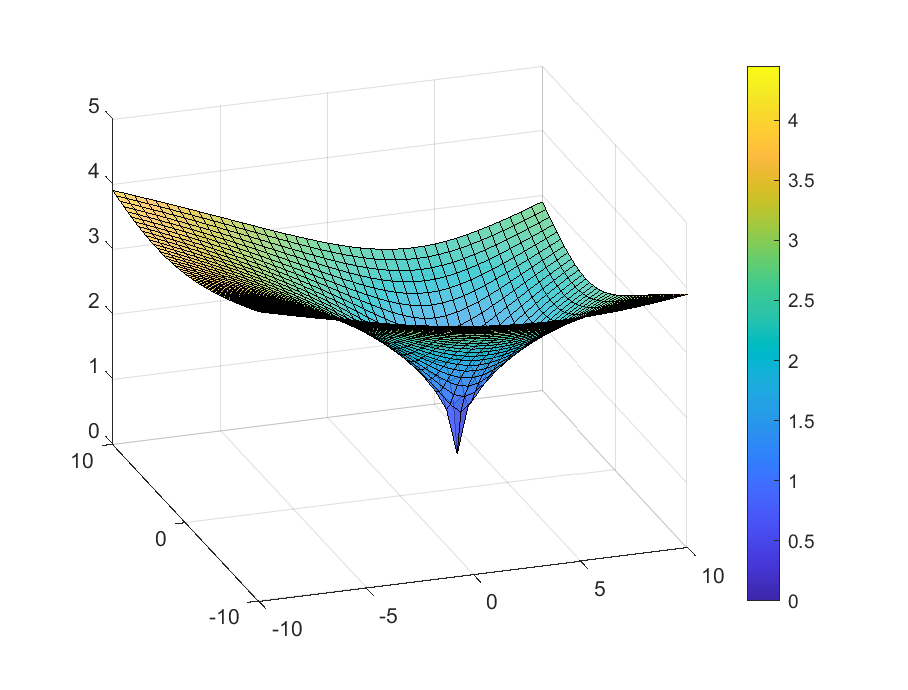
\includegraphics[scale=0.4]{figure/Q2-nondiff.eps}
\caption{Image of function \text{f\_nondiff}}
\label{fig:Q1_crite}
\end{figure}\par

\begin{figure}[h!]
\centering
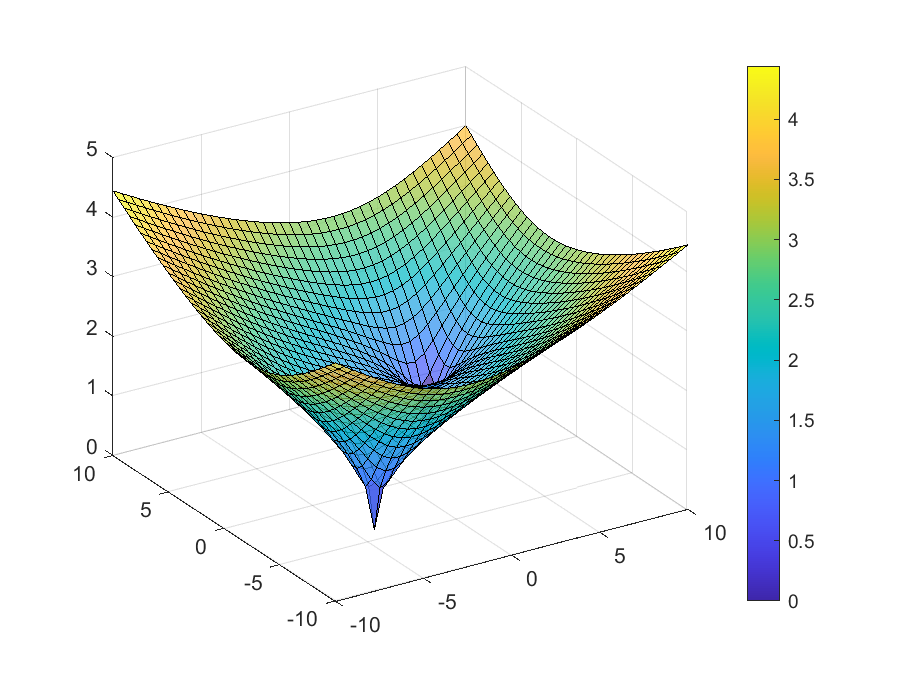
\includegraphics[scale=0.4]{figure/Q2-nondiff2.eps}
\caption{Image of function \text{f\_nondiff2}}
\label{fig:Q1_crite}
\end{figure}\par


\begin{figure}[h!]
\centering
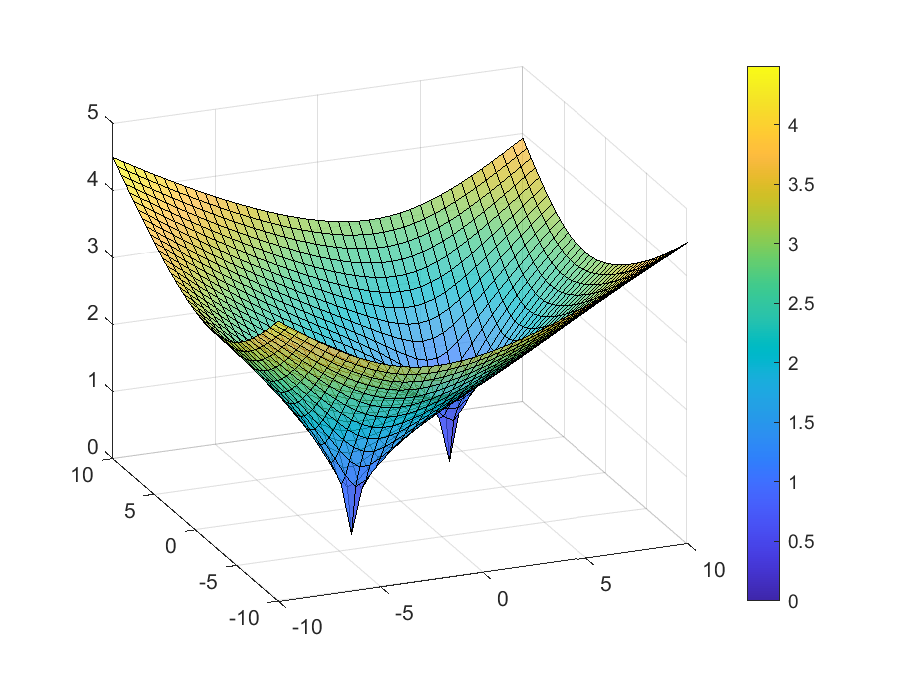
\includegraphics[scale=0.4]{figure/Q2-nondiff2asym.eps}
\caption{Image of function \text{f\_nondiff2asym}}
\label{fig:Q1_crite}
\end{figure}\par

\begin{figure}[h!]
\centering
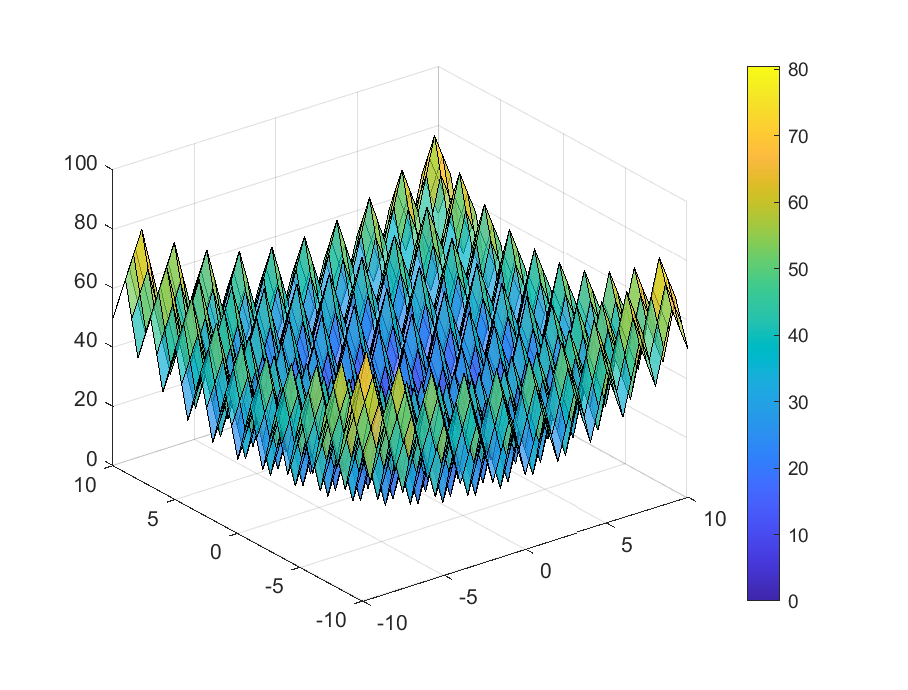
\includegraphics[scale=0.4]{figure/Q2-rastrigin.eps}
\caption{Image of function \text{f\_rastrigin}}
\label{fig:Q1_crite}
\end{figure}\par


\newpage
\section{Question 3}
First, we have the code as follows to show the behavior of $f(P_g)$
\begin{lstlisting}[style=MATLAB]
%% Behavioural analysis

figuren CRITERE
plot(1:G,min(f),'r.',1:G,max(f),'r.',...
    1:G,median(f),'m',1:G,mean(f),'b')
legend('min','max','median','mean')
title('CRITERION')
zoom on ; grid on

\end{lstlisting}
We can then get the corresponding image at figure \ref{fig:Q1_crite}.\par
\begin{figure}[h!]
\centering
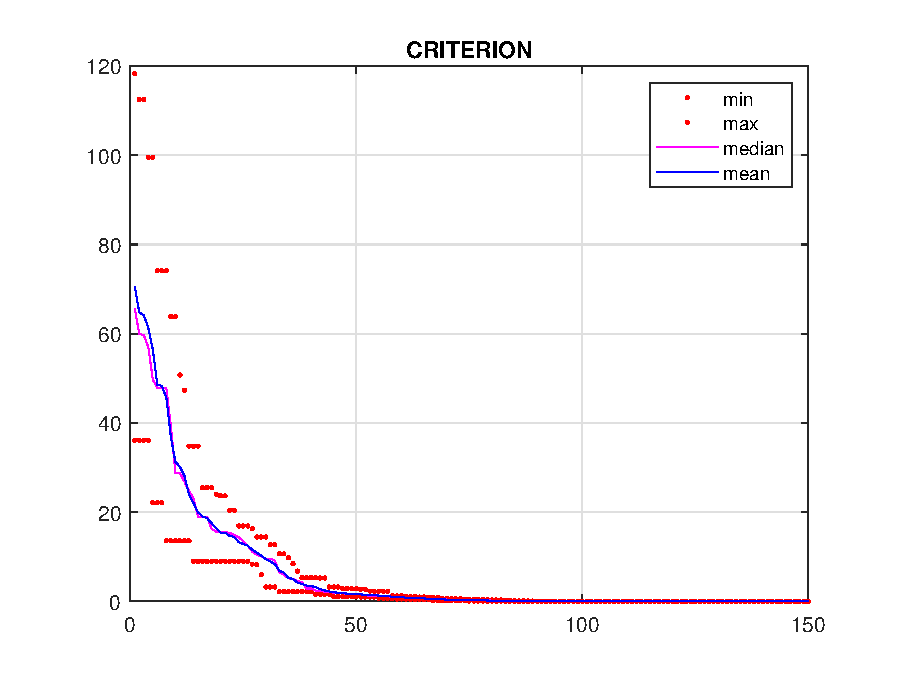
\includegraphics[scale=0.7]{figure/Q1_crite.eps}
\caption{Evolution of criterion with generation}
\label{fig:Q1_crite}
\end{figure}\par
As we can see in the figure \ref{fig:Q1_crite}, in term of function values, the first several iterations have a value extremely high, even for minimal values. As iteration goes on, the selected values converges as for each iteration. And the min and max get closer with each other. Besides, the mean value and the median value decrease, shows that almost all values converge to a minimal value.


\section{Question 4}
First, this functions mean the distance of each $x_i^{(g)}$ to the average of this iteration $\xo^{(g)}.$ The bigger the distance is, the less all values converge. If this distance decrease, it means that all value converge as iterations go on. \par
Then we have the code as follows to show the behavior of $h(P_g)$
\begin{lstlisting}[style=MATLAB]
d2mean = NaN(N,G); % Table of distances to the average position for each generation
for g=1:G
    for n=1:N
        d2mean(n,g)=norm(P(n,:,g)-mean(P(:,:,g),1));
    end
end

figuren POPULATION_stat2mean
plot(1:G,min(d2mean),'r.',1:G,max(d2mean),'r.',...
    1:G,median(d2mean),'m',1:G,mean(d2mean),'b',...
    1:G,median(d2mean)+std(d2mean),'g',1:G,max(median(d2mean)-std(d2mean),median(d2mean)/100),'g')
legend('min','max','median','mean','median+std','median-std')
title('POPULATION /mean')
zoom on ; grid on
\end{lstlisting}
We have figure \ref{fig:Q1_pop} as the output of this part of code, we can see that the median and mean value decrease which shows that the most part of point converge. Besides, the min and max get closer(median+std and median-std also get closer), which means that all values converge.
\begin{figure}[h!]
\centering
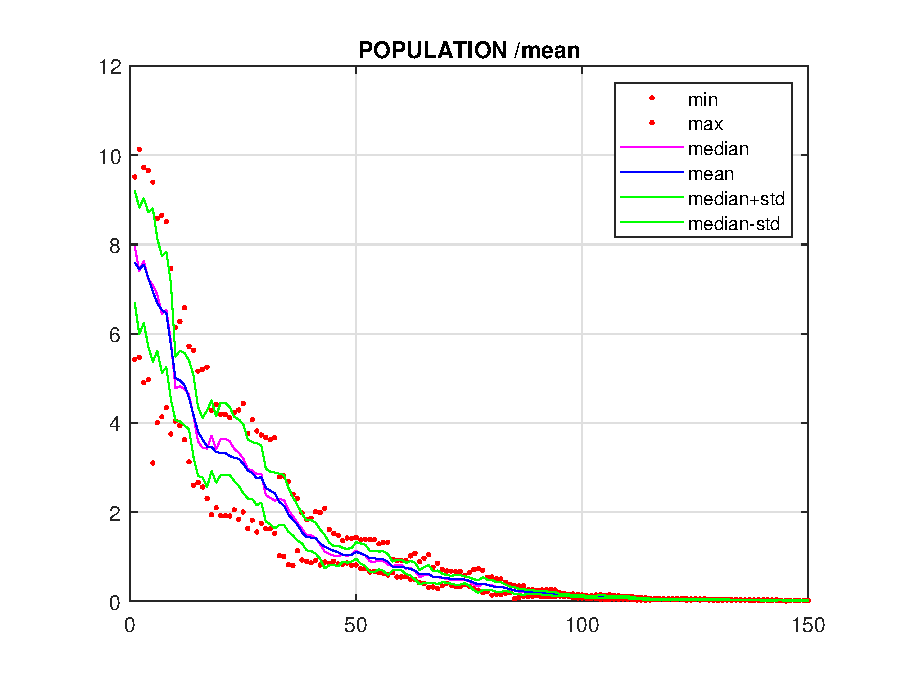
\includegraphics[scale=0.6]{figure/Q1_pop.eps}
\caption{Evolution of "converge distance" with generation}
\label{fig:Q1_pop}
\end{figure}
\section{Question 5-7}
We do a minor modification to the iteration code and we allow $G=2000$.
\begin{lstlisting}[style=MATLAB]
%% Iteration loop
G=2000;tic;
for g=1:(G-1)
    % Step 1 Mutation % THE SAME AS PREVIOUS, OMIT
    % Step 2 Crossover % THE SAME AS PREVIOUS, OMIT
    % Step 3 Selection % THE SAME AS PREVIOUS, OMIT
    if abs(min(min(f)))<0.01
        break
    end
end
calculation_time=toc;
\end{lstlisting}
And by running it for several trials, we have following solutions. We plot also the figures for the all these five trials.
\begin{lstlisting}[style=RESULT,caption={trial 1}]
=========== OPTIMAL SOLUTION
calculation time = 0.0629033s 
The iteration ends at g = 313 
The best solution is given at  314 th generation 
At index n=7 
With the value = 0.009228 
At the position = [4      3.9999           4           4           4           4           4      3.9999]
\end{lstlisting}
\begin{figure}[h!]
\centering
\begin{subfigure}[b]{0.45\textwidth}
         \centering
         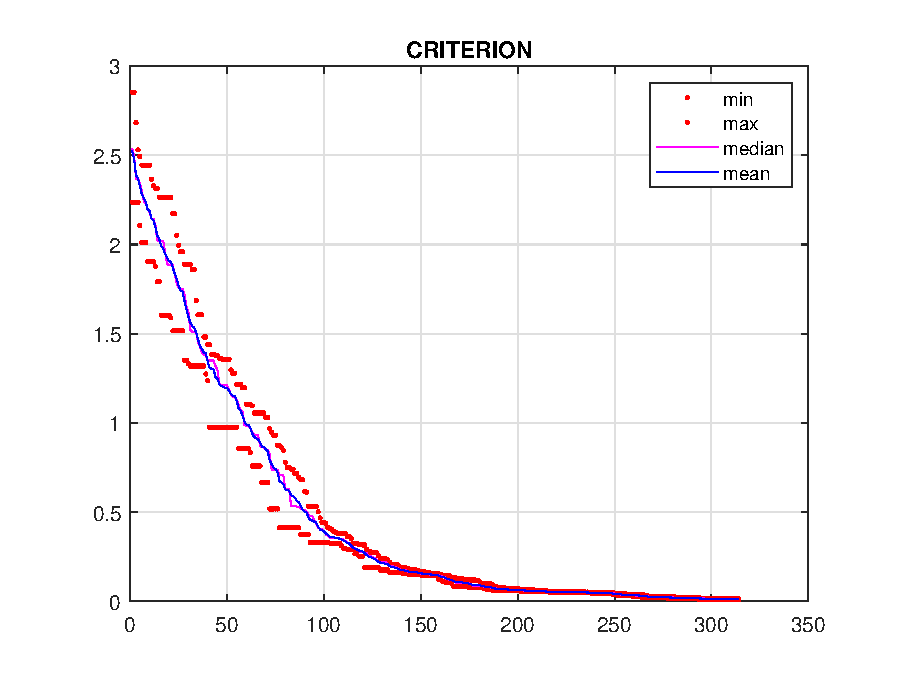
\includegraphics[scale=0.45]{figure/Q5_c1.eps}
         \caption{Criterion}
         \label{fig:Q5_c1}
     \end{subfigure}
     \hfill
     \begin{subfigure}[b]{0.45\textwidth}
         \centering
         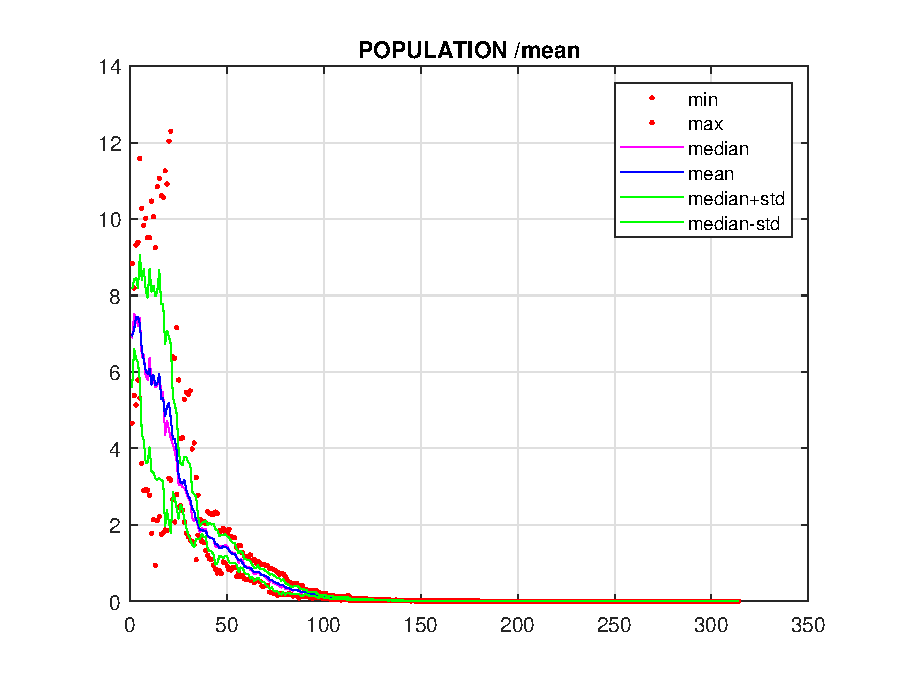
\includegraphics[scale=0.45]{figure/Q5_p1.eps}
         \caption{Distance}
         \label{fig:Q5_p1}
     \end{subfigure}
     \caption{Trial 1}
     \label{fig:trial1}
\end{figure}
\begin{lstlisting}[style=RESULT,caption={trial 2}]
=========== OPTIMAL SOLUTION
calculation time = 0.514518s 
The iteration ends at g = 1999 
The best solution is given at  515 th generation 
At index n=2 
With the value = 0.411812 (not converge!)
At the position = [3.8244      3.9945      3.9945      3.9945      3.9945      3.9945      3.9945      3.9945] 
\end{lstlisting}
\begin{figure}[h!]
\centering
\begin{subfigure}[b]{0.45\textwidth}
         \centering
         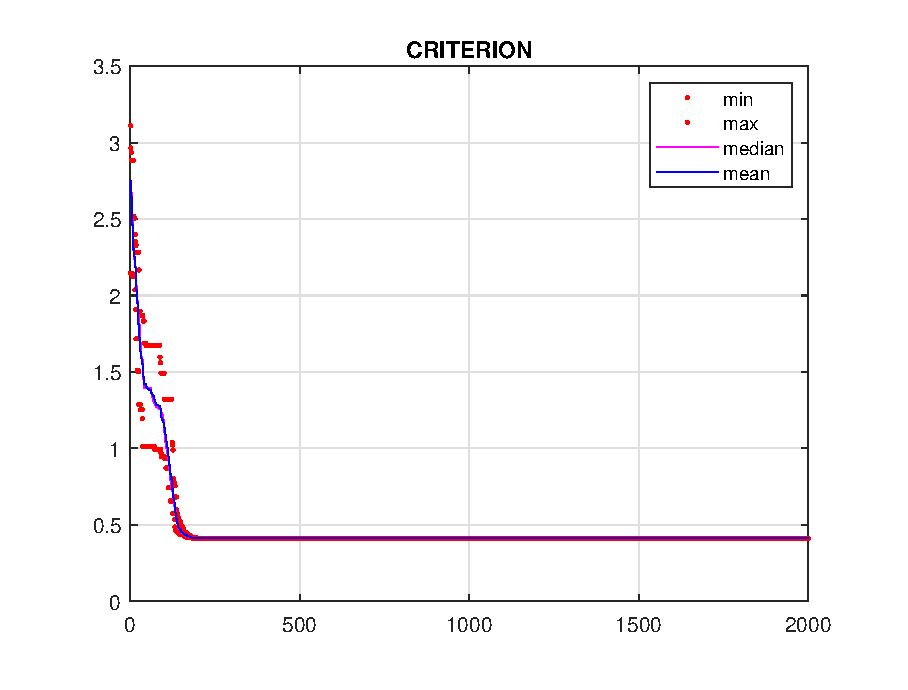
\includegraphics[scale=0.45]{figure/Q5_c2.eps}
         \caption{Criterion}
         \label{fig:Q5_c2}
     \end{subfigure}
     \hfill
     \begin{subfigure}[b]{0.45\textwidth}
         \centering
         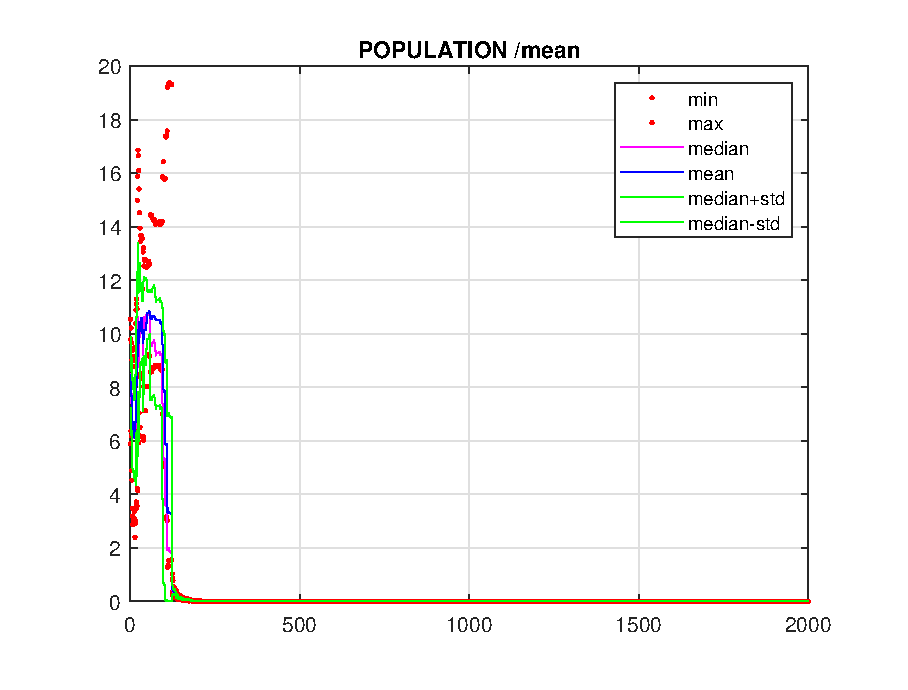
\includegraphics[scale=0.45]{figure/Q5_p2.eps}
         \caption{Distance}
         \label{fig:Q5_p2}
     \end{subfigure}
     \caption{Trial 2}
     \label{fig:trial2}
\end{figure}
\begin{lstlisting}[style=RESULT,caption={trial 3}]
=========== OPTIMAL SOLUTION
calculation time = 0.140006s 
The iteration ends at g = 261 
The best solution is given at  262 th generation 
At index n=1 
With the value = 0.009742 
At the position = [-4          -4          -4          -4          -4          -4          -4     -3.9999] 
\end{lstlisting}
\begin{figure}[h!]
\centering
\begin{subfigure}[b]{0.45\textwidth}
         \centering
         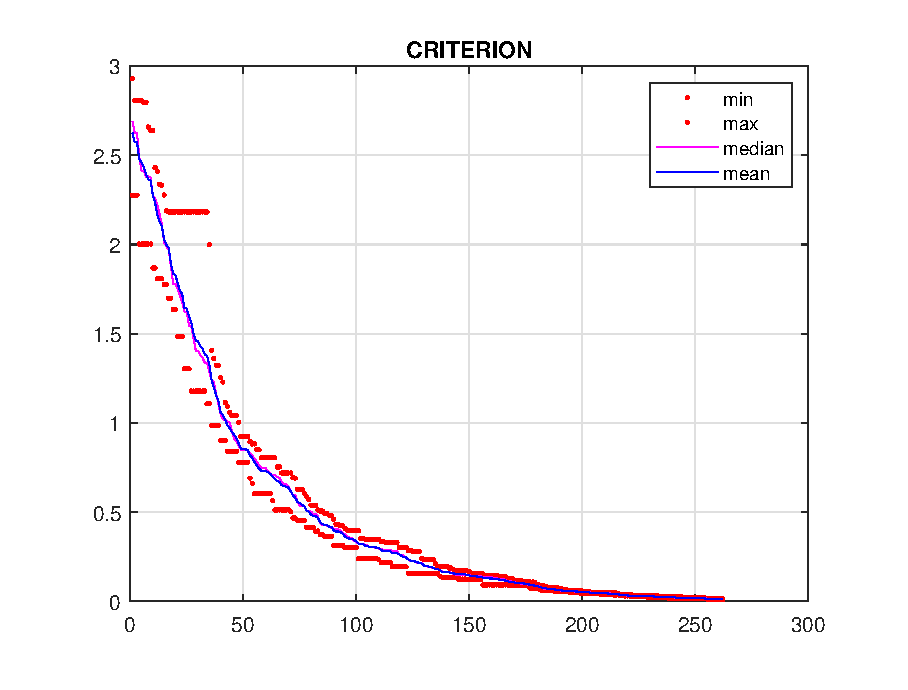
\includegraphics[scale=0.45]{figure/Q5_c3.eps}
         \caption{Criterion}
         \label{fig:Q5_c3}
     \end{subfigure}
     \hfill
     \begin{subfigure}[b]{0.45\textwidth}
         \centering
         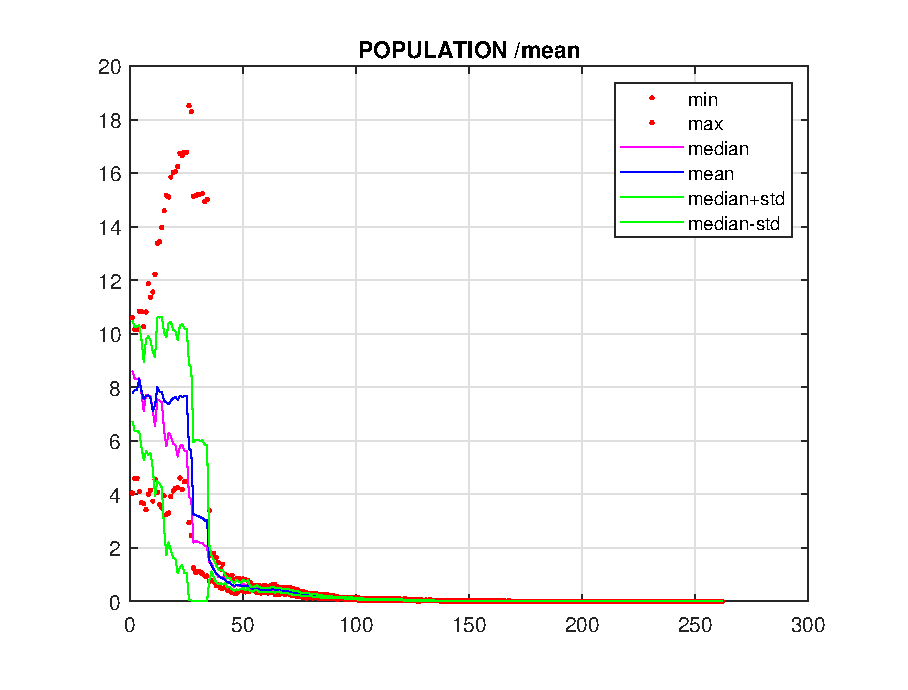
\includegraphics[scale=0.45]{figure/Q5_p3.eps}
         \caption{Distance}
         \label{fig:Q5_p3}
     \end{subfigure}
     \caption{Trial 3}
     \label{fig:trial3}
\end{figure}
\begin{lstlisting}[style=RESULT,caption={trial 4}]
=========== OPTIMAL SOLUTION
calculation time = 0.387535s 
The iteration ends at g = 1999 
The best solution is given at  369 th generation 
At index n=10 
With the value = 1.253409  (not converge!)
At the position = [3.8767      3.8767      3.8767      3.8767           5           5      3.8767      3.8767] 
\end{lstlisting}
\begin{figure}[h!]
\centering
\begin{subfigure}[b]{0.45\textwidth}
         \centering
         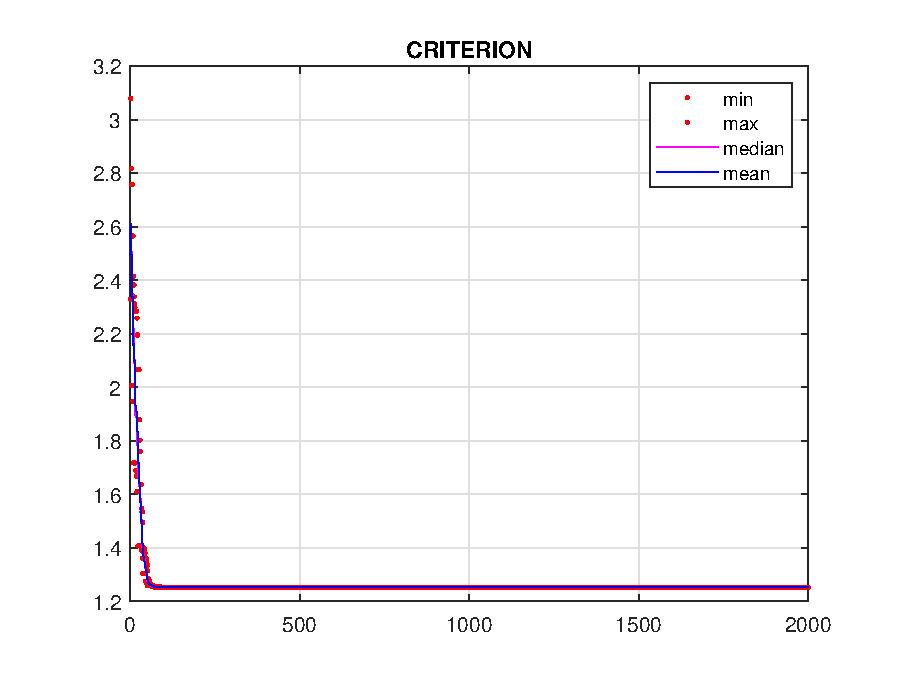
\includegraphics[scale=0.45]{figure/Q5_c4.eps}
         \caption{Criterion}
         \label{fig:Q5_c4}
     \end{subfigure}
     \hfill
     \begin{subfigure}[b]{0.45\textwidth}
         \centering
         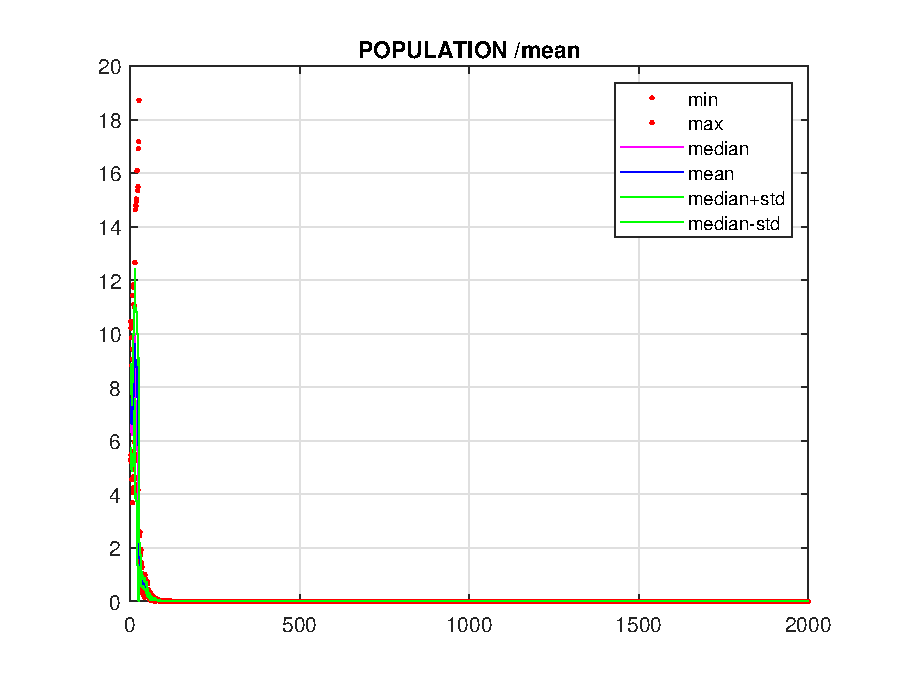
\includegraphics[scale=0.45]{figure/Q5_p4.eps}
         \caption{Distance}
         \label{fig:Q5_p4}
     \end{subfigure}
     \caption{Trial 4}
     \label{fig:trial4}
\end{figure}
\begin{lstlisting}[style=RESULT,caption={trial 5}]
=========== OPTIMAL SOLUTION
calculation time = 0.115425s 
The iteration ends at g = 303 
The best solution is given at  304 th generation 
At index n=6 
With the value = 0.009471 
At the position = [-4.0001          -4          -4     -3.9999          -4     -4.0001          -4          -4] 
\end{lstlisting}
\begin{figure}[h!]
\centering
\begin{subfigure}[b]{0.45\textwidth}
         \centering
         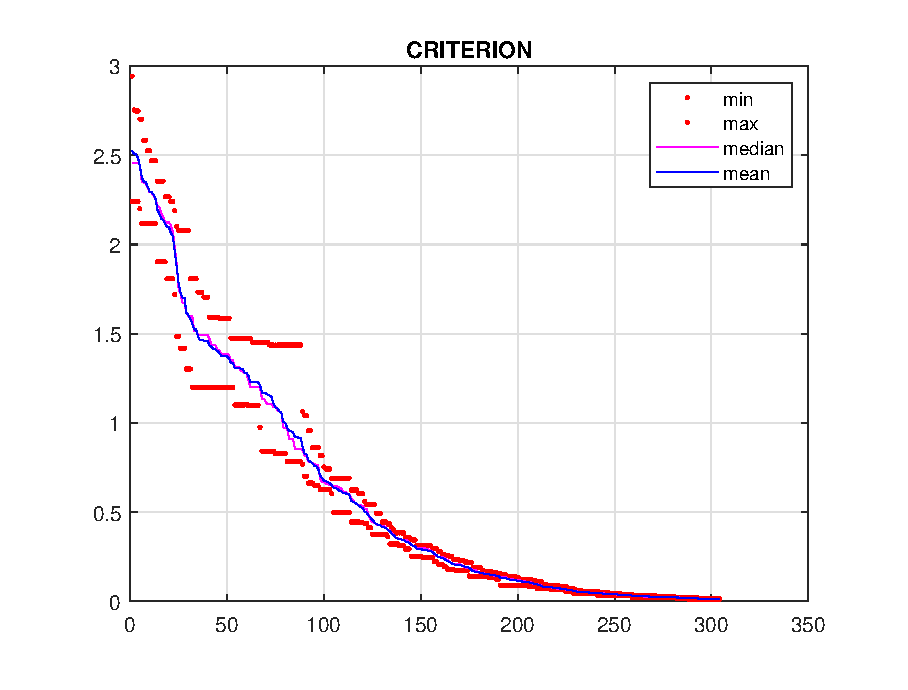
\includegraphics[scale=0.45]{figure/Q5_c5.eps}
         \caption{Criterion}
         \label{fig:Q5_c5}
     \end{subfigure}
     \hfill
     \begin{subfigure}[b]{0.45\textwidth}
         \centering
         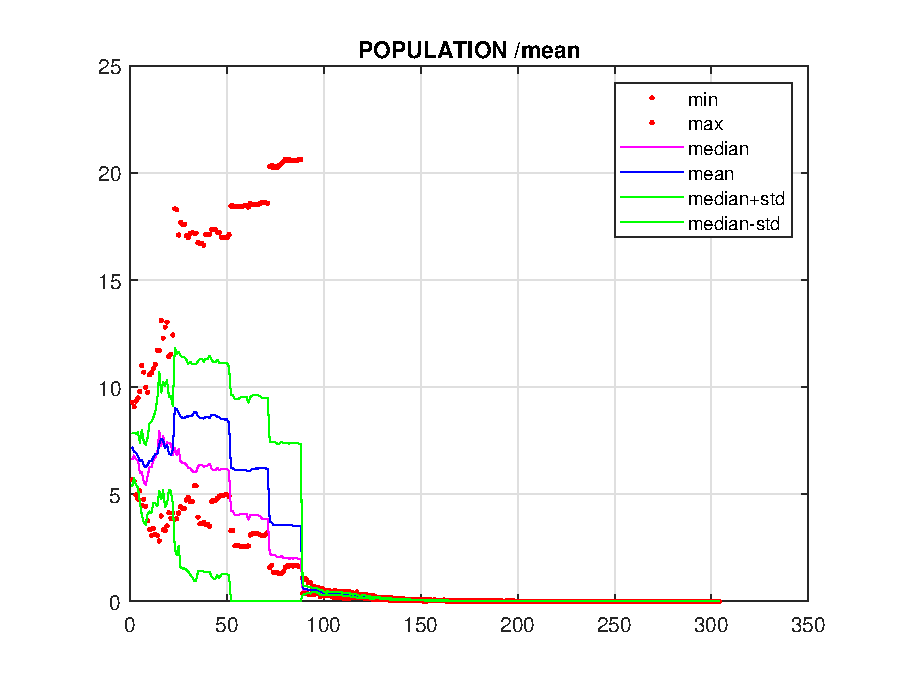
\includegraphics[scale=0.45]{figure/Q5_p5.eps}
         \caption{Distance}
         \label{fig:Q5_p5}
     \end{subfigure}
     \caption{Trial 5}
     \label{fig:trial5}
\end{figure}
Here 
As we can see, there are two trials($N^o$ 2 and 4) that never converge at the end of 2000th generation. Otherwise, it converges at around 300-400 generation, and to one of the optimal result: either $4_{1\times D}$ or $-4_{1\times D}$.

\subsection{Question 5}
\subsubsection{Performance of convergence}
As we can see in figure \ref{fig:Q5_c1}, \ref{fig:Q5_c3},\ref{fig:Q5_c5}, in case of convergence, all of $f_{optimal}$ converge to 0 as the convergence criterion is given as $|f_{optimal}-0|<0.01$, so in order to be judged as convergence, it must get sufficient close to the optimal value. However, as in figure \ref{fig:Q5_c3} and \ref{fig:Q5_c5}, we have some time the max and min values keep at a certain value for several times.
\subsubsection{Number of cases of converge}
Here we allow $G=8000$ and we do 20 trials. We want to see the total number of convergence.\par
\begin{table}[h!]
\centering
\begin{tabular}{|c|c|c|}
\hline
Total trials & Converge cases & Diverge cases \\ \hline
20           & 13             & 7             \\ \hline
\end{tabular}
\caption{Convergence and divergence count}
\end{table}
We can see that 13 out of 20 converge, so the empirical probability of converging for our parameters is about $65\%$.
\subsubsection{Code develop}
\label{code_1}
Here we evaluate if the result converge or not and the iteration needed for convergence.
\begin{lstlisting}[style=MATLAB]
%% Evaluation
cv_iters=[];
for trial=1:100
     DE_main %The main algo, the same as is given previously
     if abs(min(min(f)))>0.01
        cv_iters=[cv_iters,NaN];
     else
         cv_iters=[cv_iters,g];
     end
end
fprintf("Average convergence iteration %g \n",[mean(cv_iters,'omitnan')]) 
fprintf("Converge probability %g \n",[1-numel(cv_iters(isnan(cv_iters)))/size(cv_iters,2)]) 
\end{lstlisting}
And we get the result:
\begin{lstlisting}[style=RESULT]
Average convergence iteration 314.341 
Converge probability 0.82 
\end{lstlisting}
\subsection{Question 6}
\subsubsection{Explanation}
Let's look at figure \ref{fig:Q5_p1}, \ref{fig:Q5_p3},\ref{fig:Q5_p5}. In figure \ref{fig:Q5_p1}, the mean, median decrease almost constantly so all vectors converge quickly to the same value. But when we look at figure \ref{fig:Q5_p3},\ref{fig:Q5_p5}, we have a "plate" of blue curve(mean), red curve(max of min) and green curve(mean+std or mean-std) before a sudden converge( which will be precised in section \ref{Q7}), and even we can see some red points who goes up means that the max goes further from the optimal value for several moments.\par
But finally, we can see at least for given examples, it converge to the same solution.
\subsubsection{Statistics and MATLAB code}
\label{code_2}
Here we evaluate the final std.
\begin{lstlisting}[style=MATLAB]
%% Evaluation
final_std=[];
for trial=1:100
    DE_main %The main algo, the same as is given previously
    d2mean = NaN(N,1); % Table of distances to the average position for each generation
   for n=1:N
       d2mean(n)=norm(P(n,:,g)-mean(P(:,:,g),1));
   end
    final_std=[final_std,std(d2mean)];
end
fprintf("Average final std %g \n",[mean(final_std)]) 
\end{lstlisting}
And we get the result:
\begin{lstlisting}[style=RESULT]
Average final std 0.00251616 
\end{lstlisting}

\subsection{Question 7}
\label{Q7}
This phenomenon exists in figure \ref{fig:Q5_p3}( iterations 0-30),figure \ref{fig:Q5_p5}(iterations 20-50,50-70,70-90). The existence of this natural as the random property inside this algorithm.\par
The value of $x_{n,i}$ is to be replaced if and only if i is the active mutation or $(rand>c)$ and the newly generated $v_{n,i}$ gives a smaller value( attention, $v_{n,i}$ is also generated randomly!). In case of $x_{n,i}$ which is widely distributed, it's likely that the max value isn't changed as we always get $(rand\leq c)$ or the newly adapted value doesn't really optimize the solution. So the max value remain not changed. So finally, we can't assure that the value is changed for several iterations and so we can see the population remains very spread out before a sudden change. But attention, this is only likely to exist in case of a relatively big std.

\section{Question 8}
We merge the code of \ref{code_1} and \ref{code_2}, and we have the total schema like
\begin{lstlisting}[style=MATLAB]
clc ; clear
%% Problem settings (The same as previous)

%% Parameters for DE
N  = To change
G  = 2000;	% No. of iterations
F  = To change;	% Scaling factor
C  = To change;	% crossover probability

%% Evaluation

%MERGE OF CODE IN QUESTION 5 AND QUESTION 6

%% Output result
fprintf("Average convergence iteration %g \n",[mean(cv_iters,'omitnan')]) 
fprintf("Converge probability %g \n",[1-numel(cv_iters(isnan(cv_iters)))/size(cv_iters,2)]) 
fprintf("Average final std %g \n",[mean(final_std)]) 
\end{lstlisting}
Then let's play with the parameter!
\begin{table}[h!]
\begin{tabular}{|c|c|c|c|c|c|}
\hline
$N$                 & $F$    & $C$    & Converge probability & Average iteration & Final std \\ \hline
$\LowerInt{10+\sqrt{D}}$ & 0.8  & 0.7  &    0.75                   &     338.16                &     0.0528931        \\ \hline
$10\times D$      & 0.8  & 0.7  & 0.72                 & 318.819           & 0.0763338 \\ \hline
$D$      & 0.8  & 0.7  & 0.8                 & 320.225           & 2.01529e-05  \\ \hline
$\LowerInt{10+\sqrt{D}}$ & 0.1  & 0.7  &    0                  &     NaN               &     0.220323       \\ \hline
$\LowerInt{10+\sqrt{D}}$ & 0.5  & 0.7  &    0                  &     NaN               &     0.0122106       \\ \hline
$\LowerInt{10+\sqrt{D}}$ & 0.95 & 0.7  &                   0.68    &        428.221            &      0.0105857      \\ \hline
$\LowerInt{10+\sqrt{D}}$ & 0.8  & 0.1  &                 0.6     &         880            &       2.75855     \\ \hline
$\LowerInt{10+\sqrt{D}}$ & 0.8  & 0.98 &                 0      &           NaN        &      0.00377058      \\ \hline
\end{tabular}
\caption{Performance result by varing $N,F,C$}
\end{table}
As we can see:
\begin{itemize}
    \item For N: a bigger N will augment the average calculation time(not shown but we can feel it, as the number of calculation increase), and will decrease the probability of convergence. But it will decrease the average iteration to take and give a wider solution. This is natural as there are more values to compute at each time so there are more probability that the results go randomly to an optimal value.
    \item For F, a very small F won't even give a converge solution. A bigger F will give a more concentrated solution, but take more time to converge and are less likely to converge. It's natural as if F is vital because it influence the change at each step that we take. A too big or too small step will make the final result diverge.
    \item For C: bigger C will make the final result concentrate with each other, but won't go to optimal solution. A small $C$ make it less likely to converge and take more iterations, and it give a final result which is spread (and we may even get 2 final solution)
    
\end{itemize}
\section{Question 9-10}
It's interesting but we don't have time to play with it.
\section{Question 11}

Using the following codes, the given controller has a time-response of $0.1318$ s, an overshot of $0.5013$, a phase margin of $44.1769$, and a maximum of the control signal of $5.7441$.

\begin{lstlisting}[style=MATLAB]
%% simul_magnetic function

K =  1
Ti = 0.1
Td = 0.02
Tf = 0.001

x = log10([K, Ti, Td, Tf]);

f_simul_magnetic(x,1); % pour affichage uniquement

[stab, tr, D, delta_phi, u_max] = f_simul_magnetic(x,0) % pas d'affichage
\end{lstlisting}


\section{Question 12}
We choose this form because 
\begin{itemize}
    \item The function is positive when the closed loop is unstable and the negative, otherwise. Therefore, the minimization tends to get into the stable zone.
    \item When the closed loop is stable, the function value decreases with respect to the time-response. Therefore, the optimization tends to decrease the time-response.
\end{itemize}

To implement this, we apply the DE algorithm to the function defined by the following codes.

\begin{lstlisting}[style=MATLAB]
function f = Q12(x)
[stab, tr, D, delta_phi, u_max] = f_simul_magnetic(exp(x),0);
    if stab>0
        f=stab;
    else
        f=-1/tr;
    end
end
\end{lstlisting}

The solution is found as follows. The optimal value is -163.96, therefore, the optimal time-response is about $0.006$ s, which is much better than the previous question.

\begin{lstlisting}[style=RESULT,caption={results of Q12}]
=========== OPTIMAL SOLUTION
calculation time = 59.5814s 
The iteration ends at g = 149 
The best solution is given at  130 th generation 
At index n=1 
With the value = -163.96 
At the position = [4.8639     0.98147    0.087142   0.0025518] 
\end{lstlisting}


\begin{figure}[h!]
\centering
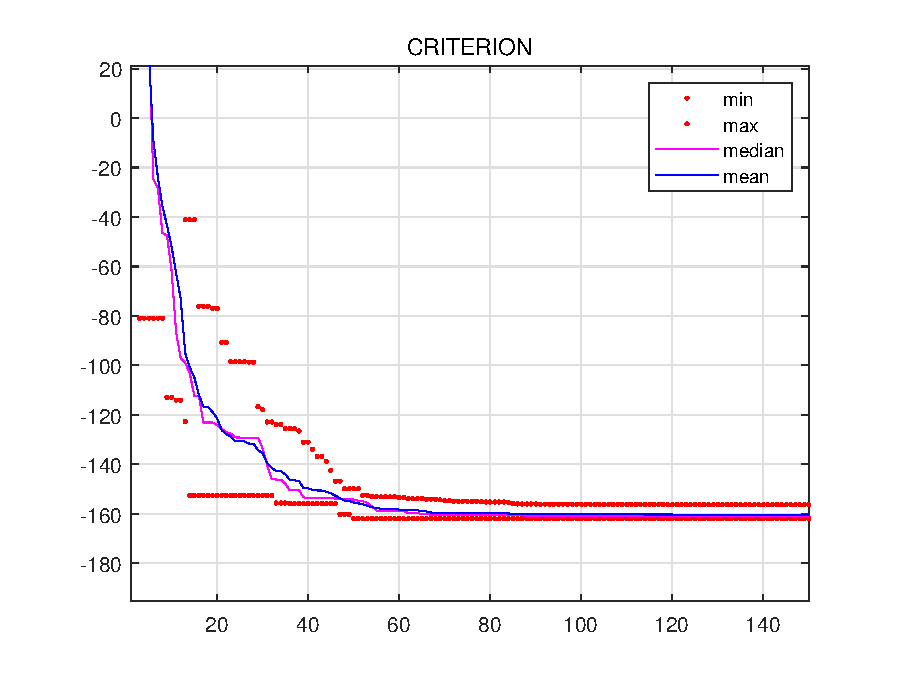
\includegraphics[scale=0.6]{figure/Q12.eps}
\caption{Evolution of function value for Q12 with generation}
\label{fig:Q1_pop}
\end{figure}


\section{Question 13}
To consider the constraint on the maximal input value, when the absolute value of input is larger than 10, $e^{\left( \lambda \frac{\max |u|-10}{10} \right)}$ increases rapidly with $u$, therefore the function value decreases with respect to $\max |u|-10$. Therefore, the algorithm tends to minimize the time-response while respecting the input constraint. 

The solution is calculated as follows. The minimal value of the function is $-2.28151$, and the associated time-response is about $0.44$ s. It can be verified that the maximal input is about 9.5, and the constraint is satisfied.
\begin{lstlisting}[style=RESULT]
=========== OPTIMAL SOLUTION
calculation time = 54.0271s 
The iteration ends at g = 149 
The best solution is given at  136 th generation 
At index n=8 
With the value = -2.28151 
At the position = [0.99869     0.61835         0.1   0.0098593] 
\end{lstlisting}

\section{Question 14}
To consider the constraint on the phase margin, using the same idea as in Q13, we can define a new cost function as
\begin{equation}
    f_3\left( x \right) =\begin{cases}
	\max \left( \mathrm{Re}\left( Poles\left( BF\left( x \right) \right) \right) \right)\\
	-\frac{1}{t_r\left( x \right) +e^{\left( \lambda \frac{\max |u\left( t \right) |-10}{10} \right)}+e^{\left( \beta \frac{45-\Delta \varphi}{45} \right)}}\\
\end{cases}
\end{equation}

The solution is calculated as follows. The minimal value of the function is $-8.21798\times10^{-24} $. However, it can be verified that the constraints are not satisfied.
\begin{lstlisting}[style=RESULT]
=========== OPTIMAL SOLUTION
calculation time = 76.3364s 
The iteration ends at g = 199 
The best solution is given at  190 th generation 
At index n=6 
With the value = -8.21798e-24 
At the position = [1.2598           1         0.1   0.0099971]

\end{lstlisting}

\begin{lstlisting}[style=RESULT]
delta_phi =20.1715
u_max =15.2977
\end{lstlisting}
\end{document}
